\documentclass[a4paper,12pt]{article}
\usepackage[T2A]{fontenc}
\usepackage[utf8]{inputenc}
\usepackage[english,russian]{babel}
\usepackage{listings}

\usepackage{amsmath}
\usepackage{MnSymbol}
\usepackage{wasysym}
\usepackage{indentfirst}
\usepackage[unicode, pdftex]{hyperref}

\usepackage{pgfplots}
\pgfplotsset{compat=1.9}

\usepackage{geometry}
\geometry{left=2cm}
\geometry{right=1.5cm}
\geometry{top=1cm}
\geometry{bottom=2cm}

\usepackage{graphicx}
\graphicspath{{img/}}
\DeclareGraphicsExtensions{.pdf,.png,.jpg}

\usepackage{float}

\newcommand{\anonsection}[1]{\section*{#1}\addcontentsline{toc}{section}{#1}}

% переименовываем  список литературы в "список используемой литературы"
\addto\captionsrussian{\def\refname{Список используемой литературы}}

\lstset{
    language=C++,
    numbers=left,
    frame=single,
    texcl=true,
    basicstyle=\ttfamily
}

\begin{document}

\begin{titlepage}

    \begin{center}
        \large
        Государственное образовательное учреждение высшего профессионального образования\\
        “Московский государственный технический университет имени Н.Э.Баумана”
        \vspace{3cm}

        \textsc{Дисциплина: Анализ алгоритмов}
        \vspace{0.5cm}

        \textsc{Лабораторная работа №5}
        \vspace{3cm}

        {\LARGE КОНВЕЕРНЫЕ ВЫЧИСЛЕНИЯ}
        \vspace{3cm}

        Студент группы ИУ7-53,\\
        Степанов Александр Олегович
        \vfill
    \end{center}

    \begin{flushright}
        \begin{tabular}{l}
            Преподаватели:\\
            Строганов Юрий Владимирович\\
            Волкова Лилия Леонидовна
        \end{tabular}
    \end{flushright}

    \begin{center}

        2019 г.

    \end{center}

\end{titlepage}

\tableofcontents

\newpage
\anonsection{Введение}

Имеется большое количество важнейших задач, решение которых требует использования огромных вычислительных мощностей, зачастую недоступных для современных вычислительных систем.

Постоянно появляются новые задачи подобного рода и возрастают требования к точности и к скорости решения прежних задач; поэтому вопросы разработки и использования сверхмощных компьютеров (называемых суперкомпьютерами) актуальны сейчас и в будущем. \cite{Voevodin} Но пока эти трудности пока что не удается преодолеть. Из-за этого приходится и эти по пути создания параллельных вычислительных систем, т.е. систем, в которых предусмотрена одновременная реализация ряда вычислительных процессов, связанных с решением одной задачи. \cite{Korneev} На современном этапе развития вычислительной техники такой способ, по-видимому, является одним из основных способов ускорения вычислений.

Многие явления природы характеризуются параллелизмом (одновременным исполнением процессов с применением различных путей и способов). В частности, в живой природе параллелизм распространен очень широко в дублирующих системах для получения надежного результата. Параллельные процессы пронизывают общественные отношения, ими характеризуются развитие науки, культуры и экономики в человеческом обществе. Среди этих процессов особую роль играют параллельные информационные потоки. \cite{Conveer}

Среди параллельных систем различают конвейерные, векторные, матричные, систолические, спецпроцессоры и т.п. В данной работе используются конвейерные. \cite{Korneev}

В данной работе стоит задача реализации алгоритма Винограда для умножения матриц, сравнение последовательной и конвейерное реализаций.

\newpage
\section{Аналитическая часть}

\subsection{Описание задачи}

Конвейеризация – это техника, в результате которой  задача или  команда разбивается  на некоторое число подзадач, которые  выполняются последовательно. Каждая  подкоманда   выполняется на своем логическом  устройстве.    Все     логические    устройства   (ступени)  соединяются последовательно таким образом, что выход  $i$-ой   ступени   связан   с   входом   $(i+1)$-ой   ступени,  все ступени  работают  одновременно.  Множество  ступеней называется    конвейером.    Выигрыш     во    времени достигается при  выполнении  нескольких задач  за  счет параллельной   работы   ступеней,  вовлекая  на  каждом такте новую задачу или команду \cite{Conveer}.

В конвейере различают $r$ последовательных этапов, так что когда $i$-я операция
проходит $s$-й этап, то $(i+k)$-я операция проходит $(s-k)$-й этап.

\begin{figure}[H]
    \center{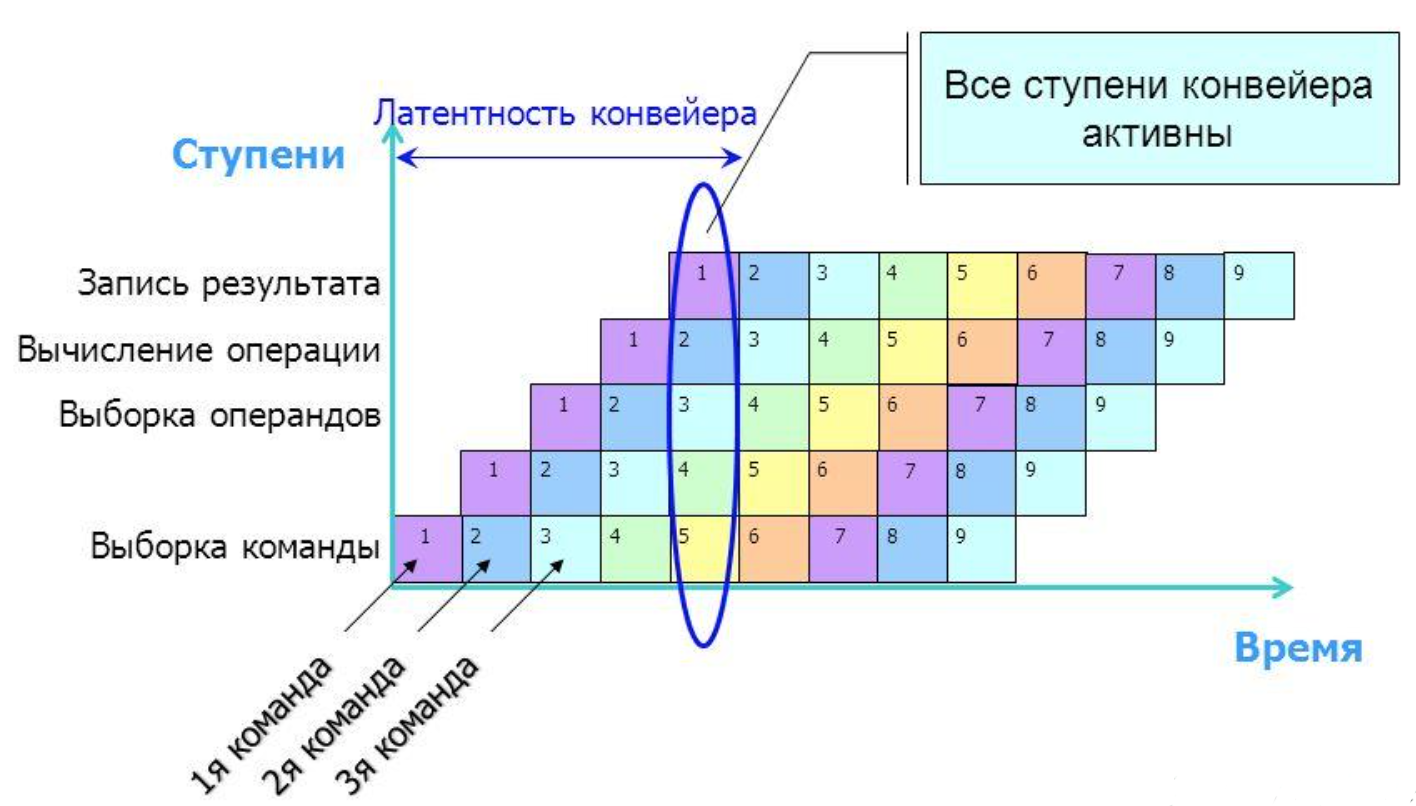
\includegraphics[scale=0.5]{conveer_img}}
    \caption{Работа конвейра}
    \label{img:conveer}
\end{figure}

\subsection{Выводы}

Таким образом, выигрыш во времени достигается при выполнении нескольких задач за
счет параллельной работы ступеней, вовлекая на каждом такте новую задачу или
команду. Однако работу конвейера тормозят зависимости  по данным и конфликты по ресурсам.

\newpage
\section{Конструкторская часть}

Рассмотрим алгоритм конвеерных вычислений для алгоритма Винограда.

\subsection{Функциональная модель}

На рисунке \ref{img:idef0} представлена функциональная модель IDEF0 уровня 1.

\begin{figure}[H]
    \center{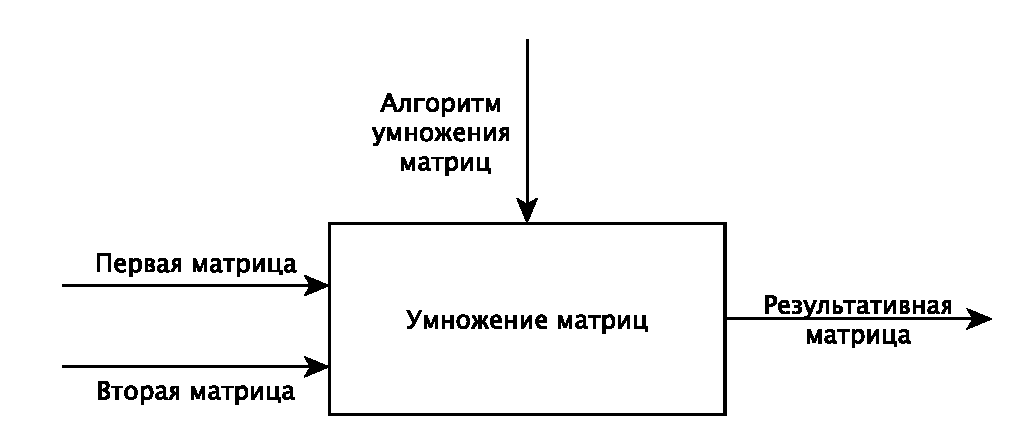
\includegraphics[scale=0.8]{IDEF0}}
    \caption{Функциональная модель IDEF0 уровня 1}
    \label{img:idef0}
\end{figure}

\subsection{Схемы алгоритмов}

На рисунке \ref{img:modvinograd} изображена схема
алгоритма Винограда.

\begin{figure}[H]
    \center{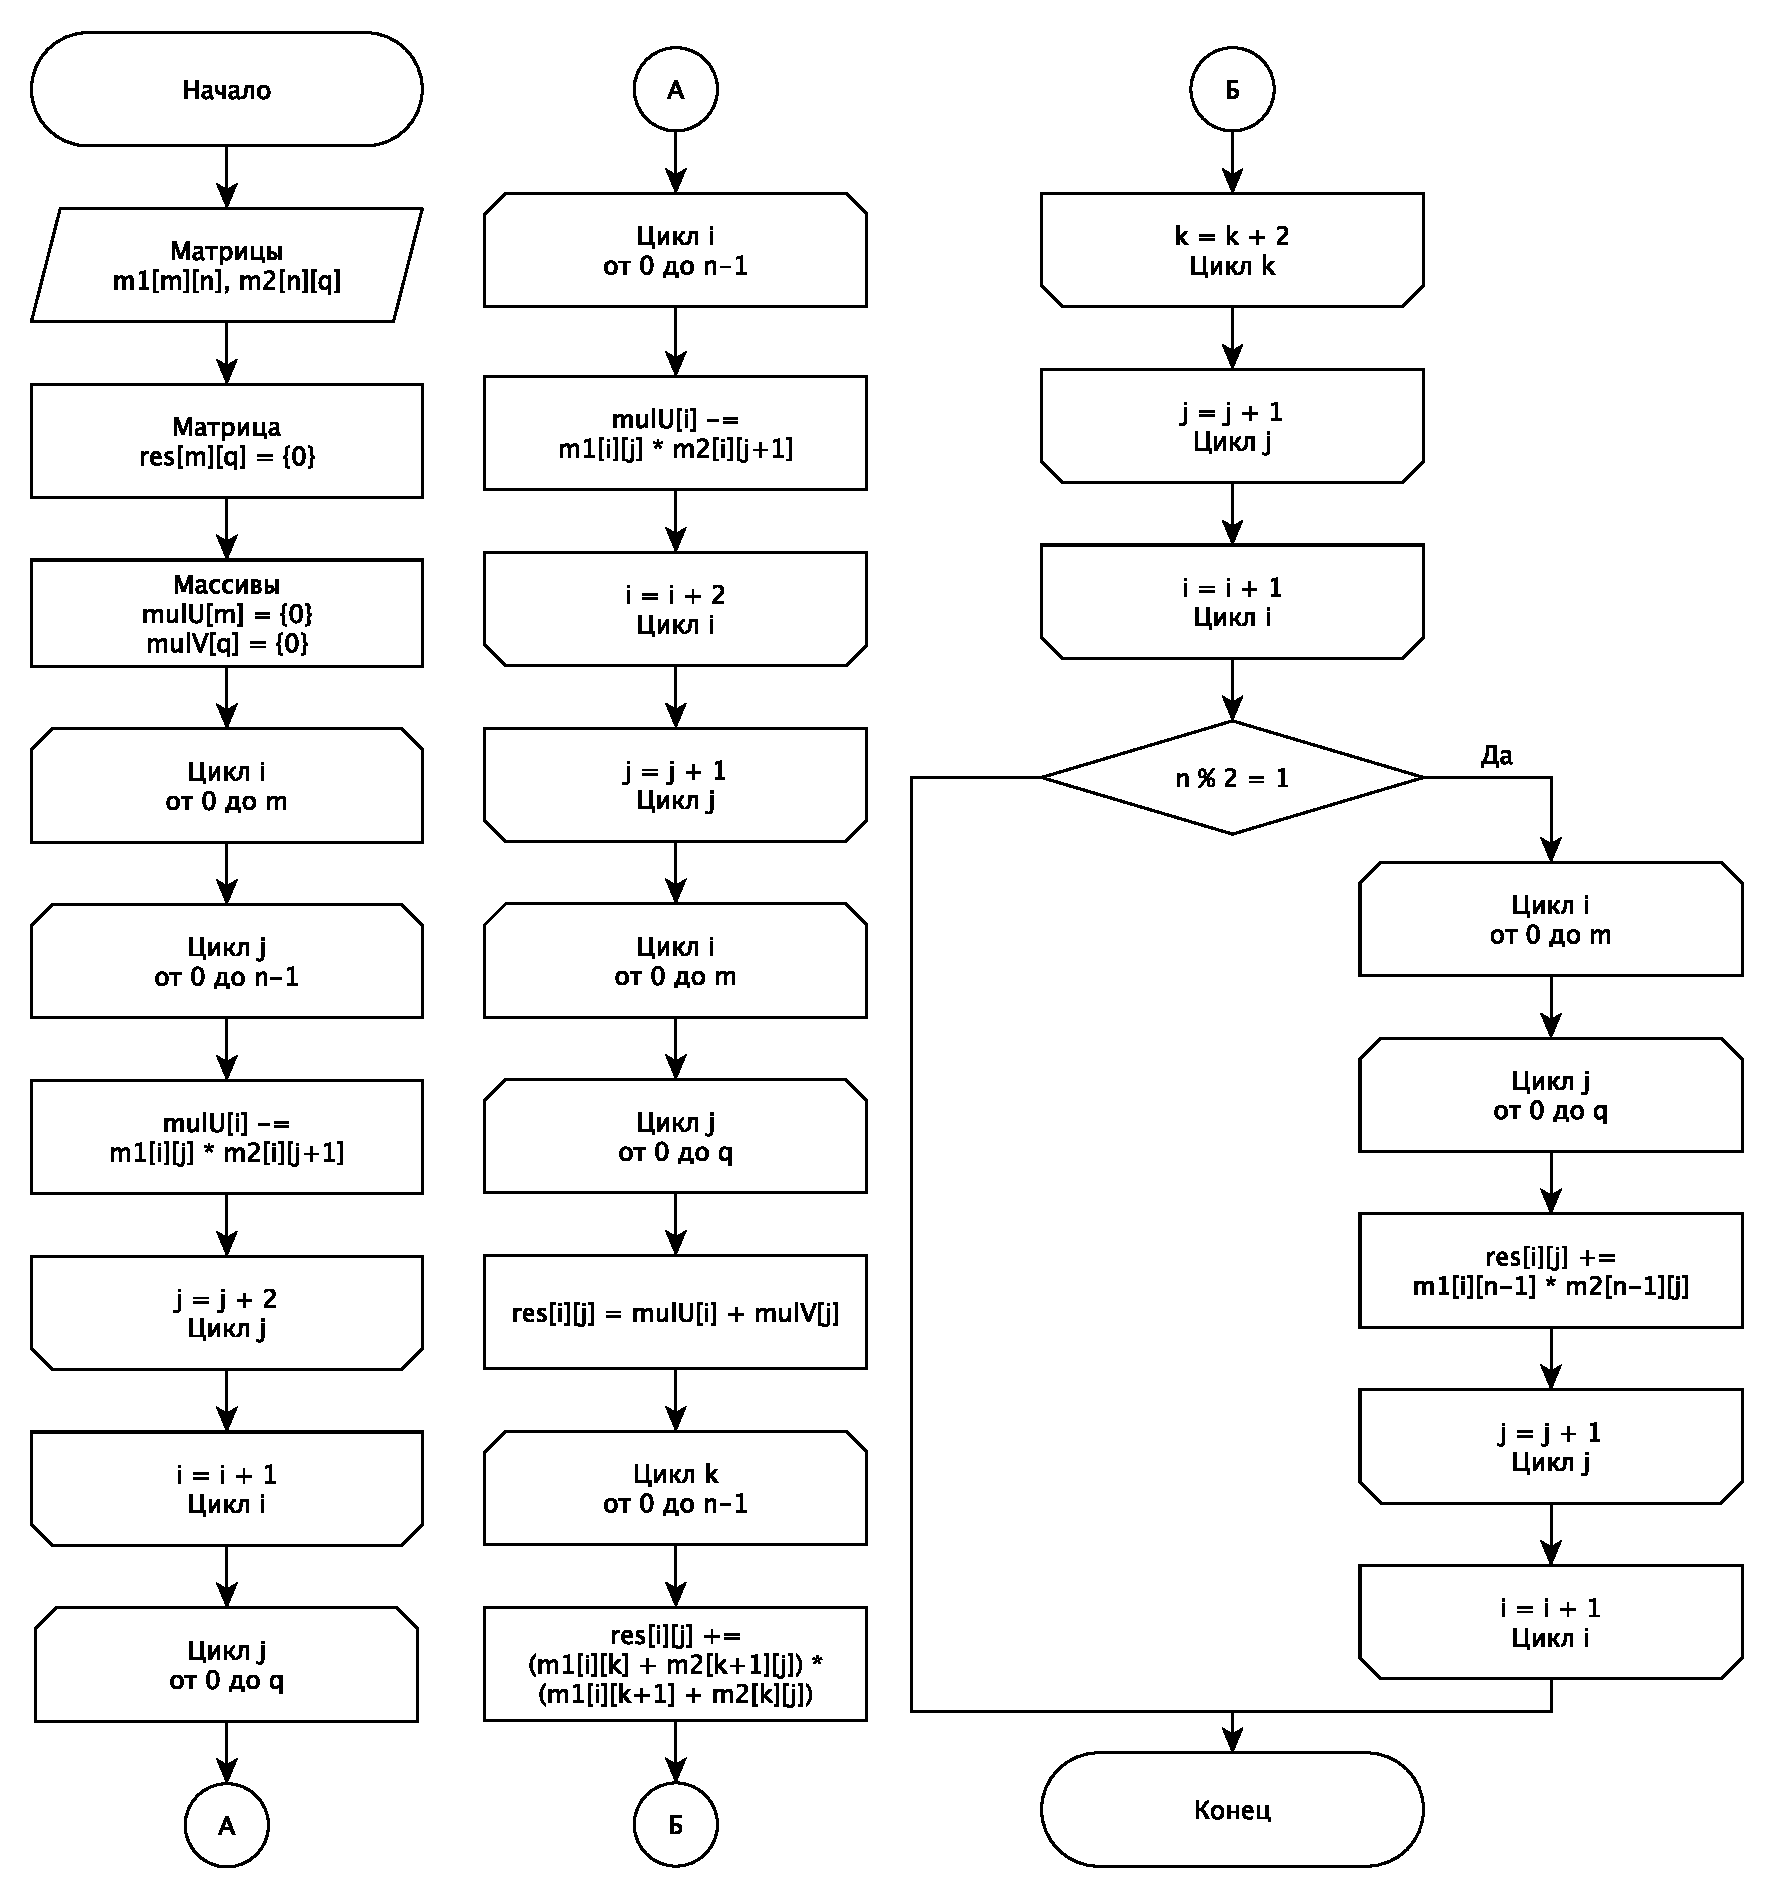
\includegraphics[scale=0.6]{modvinograd}}
    \caption{Схема алгоритма Винограда}
    \label{img:modvinograd}
\end{figure}

На рисунке \ref{img:conveer} представлена схема алгоритма, в котором действия
разделены на конвееры, выполняющиеся в отдельных потоках.

\begin{figure}[H]
    \center{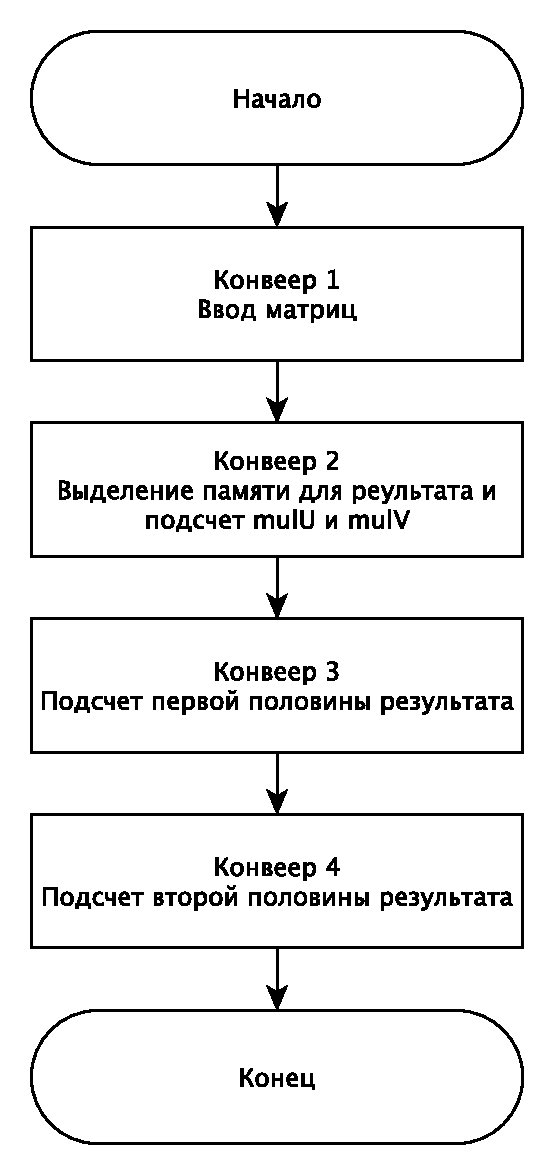
\includegraphics[scale=0.5]{conveer}}
    \caption{Схема конвейера}
    \label{img:conveer}
\end{figure}

\subsection{Выводы}

Описанный принцип построения процессора действительно напоминает конвейер сборочного завода, на котором изделие последовательно проходит ряд рабочих мест. На каждом из этих мест над изделием производится новая операция. Эффект ускорения достигается за счет одновременного выполнения частей алгоритма.

\newpage
\section{Технологическая часть}

Необходимо изучить и реализовать онвеерную разработку для умножения матриц.

\subsection{Требования к программному обеспечению}

Программное обеспечение должно обеспечивать замер процессорного времени выполнения
каждого алгоритма. Проводятся замеры для случайно генерируемых квадратных матриц
размерности до 1000.

\subsection{Средства реализации}

В качестве языка программирования был выбран {\ttfamily C++}.
Данный язык имеет высокую скорость и богатую стандартную библиотеку,
содержащую необходимые контейнеры для данной работы. Программа, написанная на
{\ttfamily C++}, будет доступна на всех платформах.

Время замерялось с помощью библиотеки {\ttfamily chrono}, которая измеряет
процессорное время \cite{chrono}. Для распараллеливания вычислений была
использована библиотека с классом нативных потоков
{\ttfamily std::thread} \cite{thread}.

Тестирование проводится на 2,7 GHz 2‑ядерном процессоре Intel Core i5 с количеством логических потоков равным 4.

\subsection{Листинг кода}

На листингах \ref{lst:inputMatrix1}, \ref{lst:inputMatrix2} предствавлен код для
выделения памяти и ввода двух матриц.

\begin{lstlisting}[caption=Ввод первой матрицы,label=lst:inputMatrix1]
void Multiplication::inputMatrix1(std::ifstream& input)
{
    input >> n1 >> m1;

    for (int i = 0; i < n1; ++i) {
        Array line;

        for (int j = 0; j < m1; ++j) {
            int element;
            input >> element;
            line.push_back(element);
        }

        first.push_back(line);
    }
}
\end{lstlisting}

\begin{lstlisting}[caption=Ввод второй матрицы,label=lst:inputMatrix2]
void Multiplication::inputMatrix2(std::ifstream& input)
{
    input >> n2 >> m2;

    for (int i = 0; i < n2; ++i) {
        Array line;

        for (int j = 0; j < m2; ++j) {
            int element;
            input >> element;
            line.push_back(element);
        }

        second.push_back(line);
    }
}
\end{lstlisting}

На листинге \ref{lst:createResult} представлен код для выделения памяти под результат
и массивы { \ttfamily mulU } и { \ttfamily mulV }.

\begin{lstlisting}[caption=Выделение памяти для результата и дополнительных массивов,label=lst:createResult]
void Multiplication::createResult()
{
    if (m1 != n2) return;

    for (int i = 0; i < n1; ++i) {
        Array line;

        for (int j = 0; j < m2; ++j) {
            line.push_back(0);
        }

        result.push_back(line);
    }

    for (int i = 0; i < n1; ++i) {
        mulU.push_back(0);
    }

    for (int i = 0; i < m2; ++i) {
        mulV.push_back(0);
    }
}
\end{lstlisting}

На листингах \ref{lst:mulU}, \ref{lst:mulV} представлен код для вычисления
массивов { \ttfamily mulU } и { \ttfamily mulV }.

\begin{lstlisting}[caption=Подсчет { \ttfamily mulU },label=lst:mulU]
void Multiplication::calcMulU()
{
    for (int i = 0; i < n1; ++i)
        for (int j = 0; j < n2 - 1; j += 2)
            mulU[i] -=
                first[i][j] * first[i][j + 1];
}
\end{lstlisting}

\begin{lstlisting}[caption=Подсчет { \ttfamily mulV },label=lst:mulV]
void Multiplication::calcMulV()
{
    for (int j = 0; j < m2; ++j)
        for (int i = 0; i < n2 - 1; i += 2)
            mulV[j] -=
                second[i][j] * second[i + 1][j];
}
\end{lstlisting}

На листингах \ref{lst:calculate1}, \ref{lst:calculate2} и \ref{lst:check} вычисляется
результат.

\begin{lstlisting}[caption=Подсчет первой половины результата,label=lst:calculate1]
void Multiplication::calculate1()
{
    for (int i = 0; i < (n1 >> 1) + 1; ++i) {
        for (int j = 0; j < m2; ++j) {
            result[i][j] = mulU[i] + mulV[j];
            for (int k = 0; k < n2 - 1; k += 2) {
                result[i][j] +=
                    (first[i][k] + second[k + 1][j]) *
                    (first[i][k + 1] + second[k][j]);
            }
        }
    }
}
\end{lstlisting}

\begin{lstlisting}[caption=Подсчет второй половины результата,label=lst:calculate2]
void Multiplication::calculate2()
{
    for (int i = (n1 >> 1) + 1; i < n1; ++i) {
        for (int j = 0; j < m2; ++j) {
            result[i][j] = mulU[i] + mulV[j];
            for (int k = 0; k < n2 - 1; k += 2) {
                result[i][j] +=
                    (first[i][k] + second[k + 1][j]) *
                    (first[i][k + 1] + second[k][j]);
            }
        }
    }
}
\end{lstlisting}

\begin{lstlisting}[caption=Проверка на нечетность и вычисление если необходимо,label=lst:check]
void Multiplication::check()
{
    if (n2 % 2 == 1)
        for (int i = 0; i < n1; ++i)
            for (int j = 0; j < m2; ++j)
                result[i][j] +=
                    first[i][n2 - 1] * second[n2 - 1][j];
}
\end{lstlisting}

На листингах \ref{lst:pipeline1}, \ref{lst:pipeline2}, \ref{lst:pipeline3} и
\ref{lst:pipeline4} проводятся конвеерные вычисления умножения матриц.

\begin{lstlisting}[caption=Первый конвейер,label=lst:pipeline1]
void Conveyor::functionPipeline1()
{
    while (true)
    {
        std::string buf;
        input >> buf;

        if (input.eof()) {
            stopPipline1 = true;
            return;
        }

        Multiplication mult;
        mult.inputMatrix1(input);
        mult.inputMatrix2(input);

        queuePipeline2.push(mult);
    }
}
\end{lstlisting}

\begin{lstlisting}[caption=Второй конвейер,label=lst:pipeline2]
void Conveyor::functionPipeline2()
{
    while (true)
    {
        if (stopPipline1 &&
            queuePipeline2.empty()) {
            stopPipline2 = true;
            return;
        }

        if (queuePipeline2.empty()) continue;

        Multiplication mult = queuePipeline2.front();
        queuePipeline2.pop();

        mult.createResult();
        mult.calcMulU();
        mult.calcMulV();

        queuePipeline3.push(mult);
    }
}
\end{lstlisting}

\begin{lstlisting}[caption=Третий конвейер,label=lst:pipeline3]
void Conveyor::functionPipeline3()
{
    while (true)
    {
        if (stopPipline2 &&
            queuePipeline3.empty()) {
            stopPipline3 = true;
            return;
        }

        if (queuePipeline3.empty()) continue;

        Multiplication mult = queuePipeline3.front();
        queuePipeline3.pop();

        mult.calculate1();

        queuePipeline4.push(mult);
    }
}
\end{lstlisting}

\begin{lstlisting}[caption=Четвертый конвейер,label=lst:pipeline4]
void Conveyor::functionPipeline4()
{
    while (true)
    {
        if (stopPipline3 &&
            queuePipeline4.empty()) {
            return;
        }

        if (queuePipeline4.empty()) continue;

        Multiplication mult = queuePipeline4.front();
        queuePipeline4.pop();

        mult.calculate2();
        mult.check();

        queueResult.push(mult);
    }
}
\end{lstlisting}

\subsection{Тестирование}

Для тестирования программы были заготовлены следующие тесты в таблице
\ref{table:test}.

\begin{table}[H]
    \caption{Тесты для алгоритмов}
    \label{table:test}
    \centering
    \begin{tabular}{|c|c|c|}
        \hline
        Первая матрца & Вторая матрица & Ожидаемый результат \\
        \hline
        1 2 & 1 2 & \ 7 10 \\
        3 4 & 3 4 & 15 22 \\
        \hline
        1 2 3 & 1 2 3 & \ 30\ \ 36\ \ 42 \\
        4 5 6 & 4 5 6 & \ 66\ \ 81\ \ 96 \\
        7 8 9 & 7 8 9 & 102 126 150 \\
        \hline
        1 2 3 & 1 & 14 \\
        4 5 6 & 2 & 32 \\
              & 3 & \\
        \hline
    \end{tabular}
\end{table}

\subsection{Выводы}

Для исследования конвеерных вычислений был реализован алгоритм на выбранном языке
{ \ttfamily C++ }. Чтобы проверить правильность работы были подготовлены тесты.

\newpage
\section{Экспериментальная часть}

Проведем тестирование и сравним алгоритмы по времени работы.

\subsection{Примеры работ}

На рисунках \ref{img:zero}, \ref{img:nef} и \ref{img:good} изображены примеры работ.

\begin{figure}[H]
    \centering
    
\includegraphics[scale=0.4]{zero_arg}
    \caption{Нет аргументов}
    \label{img:zero}
\end{figure}

\begin{figure}[H]
    \centering
    
\includegraphics[scale=0.4]{non_exist_file}
    \caption{Несуществующий файл}
    \label{img:nef}
\end{figure}

\begin{figure}[H]
    \centering
    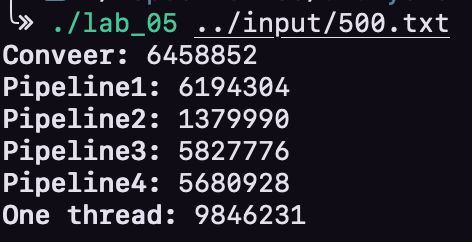
\includegraphics[scale=0.8]{good}
    \caption{Успешное выполнение}
    \label{img:good}
\end{figure}

\subsection{Результаты тестирования}

Для тестирования были использованы тесты в таблице \ref{table:test}.
Результаты продемонстрированы в таблице\ref{table:test-res}.

\begin{table}[H]
    \caption{Результаты тестирования}
    \label{table:test-res}
    \centering
    \begin{tabular}{|c|c|c|}
        \hline
        Первая матрца & Вторая матрица & Результат \\
        \hline
        1 2 & 1 2 & \ 7 10 \\
        3 4 & 3 4 & 15 22 \\
        \hline
        1 2 3 & 1 2 3 & \ 30\ \ 36\ \ 42 \\
        4 5 6 & 4 5 6 & \ 66\ \ 81\ \ 96 \\
        7 8 9 & 7 8 9 & 102 126 150 \\
        \hline
        1 2 3 & 1 & 14 \\
        4 5 6 & 2 & 32 \\
              & 3 & \\
        \hline
    \end{tabular}
\end{table}

Все тесты пройдены успешно.

\subsection{Замеры времени}

На рисунке \ref{img:graph} видно сравнение времени работы одного потока простив
конвейра на примере количества матриц от 100 до 1000.

\begin{figure}[H]
    \begin{tikzpicture}
        \begin{axis}[
            legend pos = north west,
            xlabel=Количество матриц,
            ylabel=микросекунды,
            grid = major,
            width = 0.8\paperwidth,
            height = 0.38\paperheight,
            line width = 1
        ]
            \legend{
                1 поток,
                Конвейер
            };

            \addplot coordinates {
                (100, 1979087)
                (200, 3938924)
                (300, 5899570)
                (400, 7890858)
                (500, 9846231)
                (600, 11803949)
                (700, 13777380)
                (800, 15747592)
                (900, 17697605)
                (1000, 19764128)
            };

            \addplot coordinates {
                (100, 1320171)
                (200, 2604349)
                (300, 3869893)
                (400, 5201684)
                (500, 6458852)
                (600, 7579206)
                (700, 8869803)
                (800, 10116102)
                (900, 11475725)
                (1000, 12852206)
            };
        \end{axis}
    \end{tikzpicture}
    \caption{Сравнение конвейра с 1 потоком}
    \label{img:graph}
\end{figure}

\subsection{Выводы}

Конвейерная реализация выигрывает у обычной примерно в да раза (рисунок \ref{img:graph}).

\newpage
\anonsection{Заключение}

Таким образом, выигрыш во времени достигается при  выполнении нескольких задач за счет параллельной   работы   ступеней,  вовлекая  на  каждом такте новую задачу или команду.

В результате проведенныъх исслевований был реализован алгоритм Винограда, распараллеленный
по конвейрам. В результате такой алгоритм оказался быстрей в два раза, чем обычный.
Ускорение произошло благодаря одновременного выполнения частей алгоритма.

\newpage
\addcontentsline{toc}{section}{Список используемой литературы}

\begin{thebibliography}{}
    \bibitem{chrono} Документация по chrono [Электронный ресурс]. -
    Режим доступа: http://www.cplusplus.com/reference/chrono/
    Дата обращения: 08.10.2019
    \bibitem{thread} Документация по thread [Электронный ресурс]. -
    Режим доступа: https://ru.cppreference.com/w/cpp/thread/thread
    Дата обращения: 21.10.2019
    \bibitem{Voevodin} Воеводин В.В. Математические модели и методы в параллельных процессах. М., 1986. 296 с.
    \bibitem{Korneev} Корнеев В.В. Параллельные вычислительные системы. М., 1999. 320 с.
    \bibitem{Yukiya} Yukiya Aoyama, Jun Nakano. RS/6000 SP:Practical MPI Programming. IBM. Technical Support Organization., 2000. 221
    \bibitem{Conveer} Конвеерные вычисления [Электронный ресурс]. - Режим доступа: http://www.myshared.ru/slide/674082/(дата обращения: 03.12.2019)
    \bibitem{recursive} Применение модели конвейерных процессов рекурсивного типа для решения прикладных задач [Электронный ресурс] - Режим доступа: https://cyberleninka.ru/article/n/primenenie-modeli-konveyernyh-protsessov-rekursivnogo-tipa-dlya-resheniya-prikladnyh-zadach Дата обращения: 03.12.2019
\end{thebibliography}

\end{document}
